\chapter{Архитектура приложения}
\label{cha:design}

\section{Общая архитектура}

Приложение построено по клиент-серверной архитектуре с единым API-контрактом. Центральным элементом является OpenAPI~3.0 спецификация~\cite{openapi:spec}, описывающая все эндпоинты, типы данных и форматы ответов REST API.

Система состоит из нескольких компонентов:
\begin{enumerate}
\item \textbf{Сервер} (Go)---обработка HTTP-запросов, бизнес-логика, работа с базой данных;
\item \textbf{Десктопный клиент} (C++/Qt6)---нативное приложение для диспетчера;
\item \textbf{Веб-интерфейс} (React/TypeScript)---публичное приложение для студентов.
\end{enumerate}

\section{Серверная часть (Go)}

Серверная часть использует слоистую архитектуру:
\begin{itemize}
\item \textbf{Слой API}---автоматически сгенерированные типы и интерфейс StrictServerHandler (oapi-codegen)~\cite{oapi:codegen};
\item \textbf{Слой приложения} (Application)---реализация бизнес-логики и хендлеров REST-эндпоинтов;
\item \textbf{Слой репозитория} (Repository)---работа с базой данных через sqlc~\cite{sqlc:dev};
\item \textbf{Слой библиотек} (Lib)---парсер XLSX, сериализатор ICS.
\end{itemize}

Запуск сервера осуществляется в \Code{main.go}: загрузка конфигурации, подключение к PostgreSQL~\cite{postgres:doc}, создание Application, оборачивание в StrictHandler, запуск HTTP-сервера.

\section{Десктопный клиент (C++/Qt6)}

Десктопный клиент реализован на C++20 с использованием Qt~6~\cite{qt:doc}.

На рисунке~\ref{fig:uml} представлена диаграмма классов десктопного клиента.

\begin{figure}[H]
  \centering
  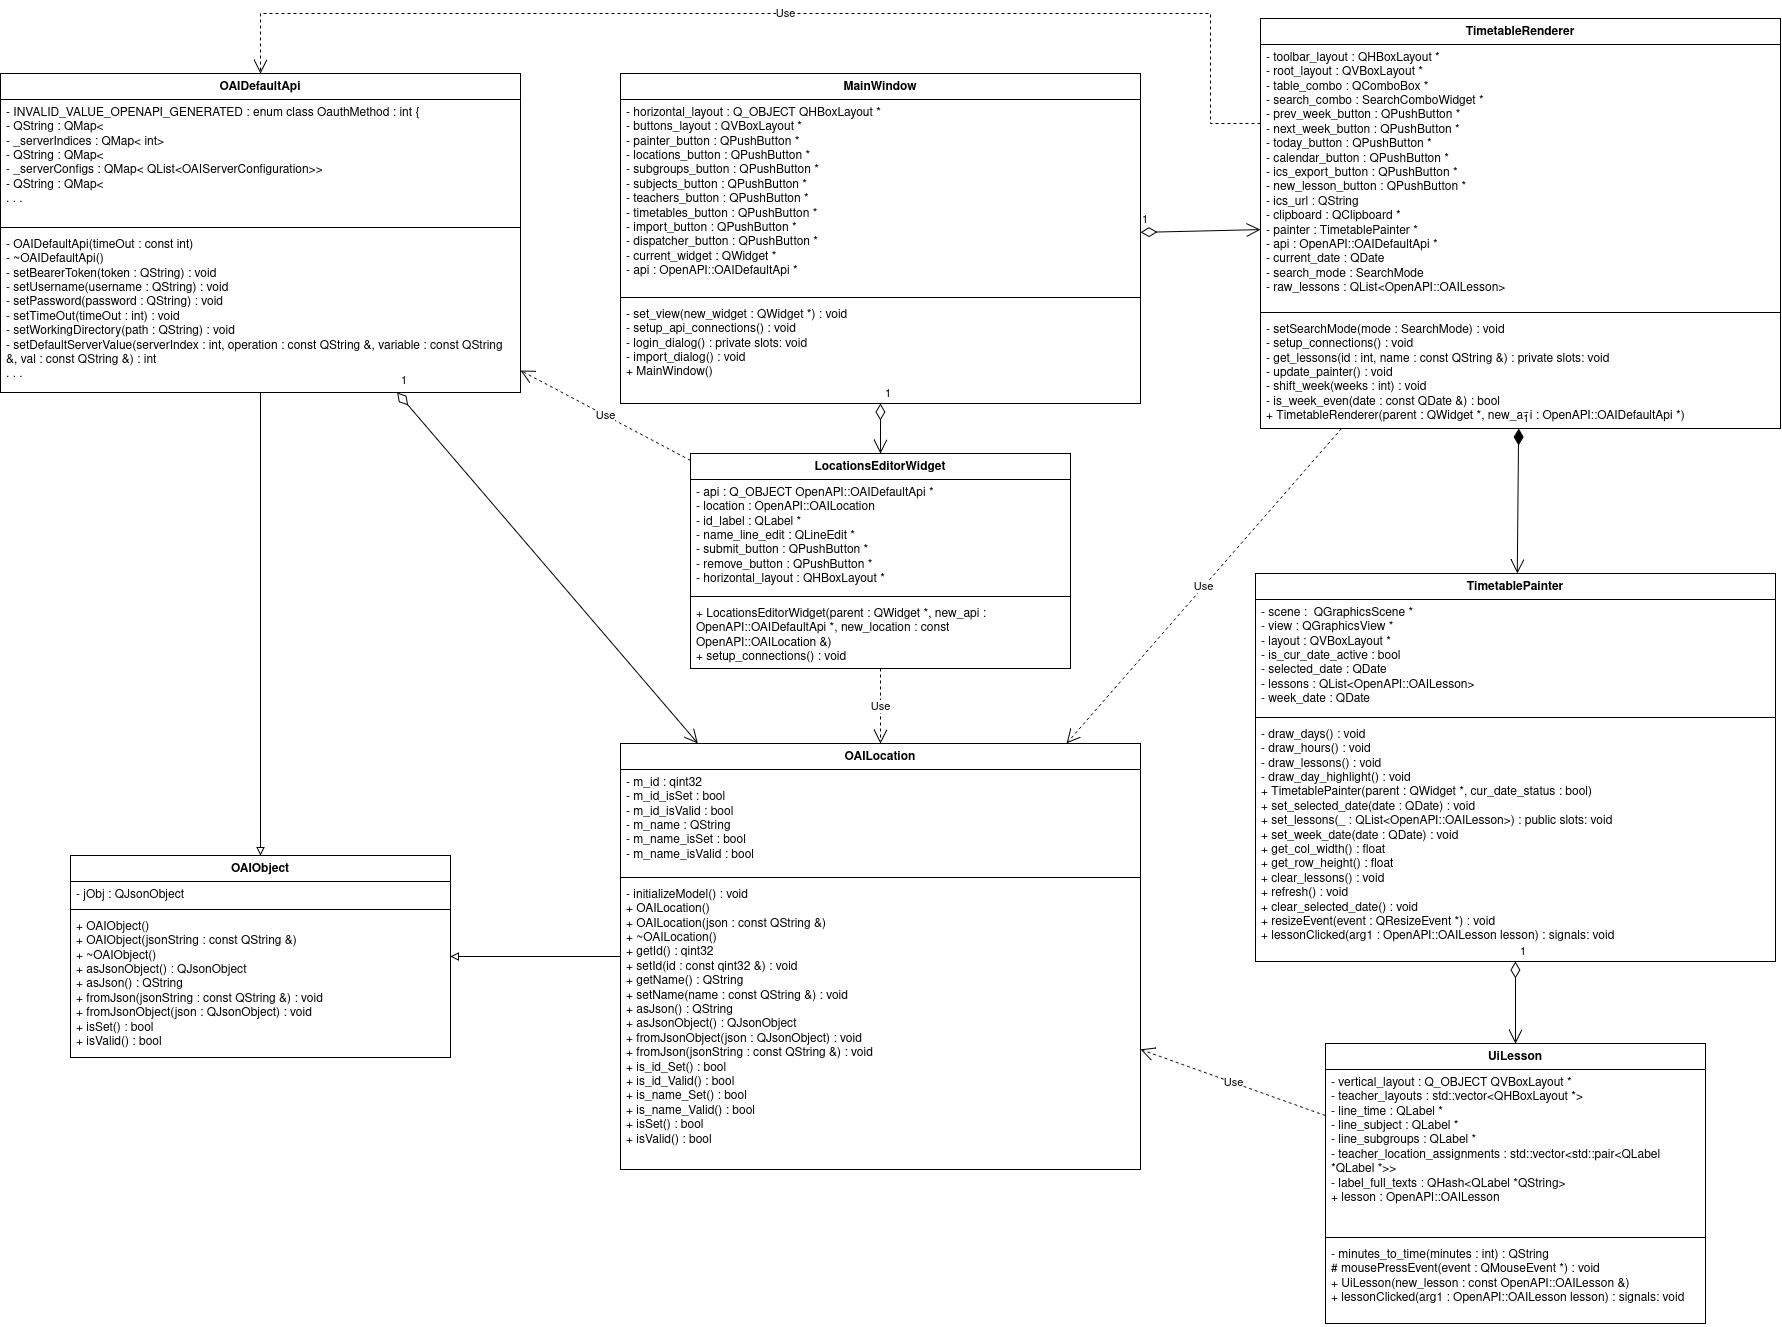
\includegraphics[width=\textwidth]{arm.drawio.png}
  \caption{Диаграмма классов десктопного клиента}
  \label{fig:uml}
\end{figure}

Основные компоненты и связи между ними:
\begin{itemize}
\item \textbf{MainWindow}---главное окно приложения, агрегирует TimetableRenderer и LocationsEditorWidget;
\item \textbf{TimetableRenderer}---виджет просмотра расписания с панелью инструментов; использует OAIDefaultApi для получения данных; композиционно владеет TimetablePainter;
\item \textbf{TimetablePainter}---отрисовка недельной сетки расписания средствами QGraphicsScene/QGraphicsView; агрегирует UiLesson; зависит от OAILocation;
\item \textbf{LocationsEditorWidget}---виджет редактирования аудиторий; зависит от OAIDefaultApi;
\item \textbf{OAIDefaultApi}---сгенерированный по OpenAPI-спецификации класс для взаимодействия с REST API; наследуется от OAIObject;
\item \textbf{OAILocation}---модель данных локации; наследуется от OAIObject.
\end{itemize}

Аналогичную структуру имеют редакторы SubgroupEditorWidget, TeacherEditorWidget, SubjectEditorWidget, предназначенные для редактирования подгрупп, преподавателей и дисциплин соответственно. Каждый из них зависит от OAIDefaultApi и построен по тому же принципу, что и LocationsEditorWidget.

\section{Структура базы данных}

База данных реализована средствами PostgreSQL~16 и включает таблицы: \Code{subgroups}, \Code{teachers}, \Code{locations}, \Code{subjects}, \Code{timetables}, \Code{lessons}, \Code{subgroup\_assignments}, \Code{teacher\_location\_assignments}. Миграции выполняются с помощью goose~\cite{goose:migrate}, генерация type-safe запросов---с помощью sqlc~\cite{sqlc:dev}.
